\documentclass{article}
\usepackage{iclr2021,times}
\iclrfinalcopy % Camera ready version!

\usepackage[utf8]{inputenc}
\usepackage[T1]{fontenc}

\usepackage[hyphens]{url}
\usepackage{hyperref}
\usepackage{graphicx}
\hypersetup{
    colorlinks,
    citecolor=blue,
    filecolor=blue,
    linkcolor=blue,
    urlcolor=blue,
}
\usepackage{algorithm}
\usepackage{algorithmic} 

\usepackage{natbib}
\setcitestyle{authoryear,open={(},close={)}}

\usepackage{amsmath,amssymb}
\usepackage{makecell}
\usepackage{chngcntr} % make figure numbering in appendix work

\usepackage{caption}
% Small captions
\captionsetup[figure]{font=small,labelfont=small}

%%% SPACE-REDUCING HACK 1/2
% Reduce spacing around floats 
\setlength{\floatsep}{8pt plus 4pt minus 4pt}
\setlength{\textfloatsep}{8pt plus 4pt minus 3pt}

\usepackage{xcolor}


\title{Planetary Nebulae Classification from Limited Labeled Dataset \\ Checkpoint 1}
\author{Joseph Hadidjojo \And Tung Pham \And Arman Muratbayev}

\begin{document}

\maketitle

% \textbf{Instructions for Checkpoint 1:} ~~\url{https://www.cs.tufts.edu/cs/152L3D/2024f/project_checkpoint1.html}


\section*{A: Changelog}

Since the last milestone (project pitch), we have changed:
\begin{itemize}
    \item Refined Dataset selection to one constant Modality (SSS Optical Images*) \\ *SSS: SuperCOSMOS Sky Survey
    \item Added Pseudo-labeling as an additional method in consideration (in addition to LP-FT)
\end{itemize}

\section*{B: Challenges}
At the moment, our biggest roadblocks are:
\begin{enumerate}
    \item Dataset scrapping (70\% done) \& Split Formulation.
    \item Testing initial code implementation on the HPC (to gauge required computing time)
    \item Ratifying the best method to implement Pseudo-labeling to our specific dataset
\end{enumerate}

We'd like instructor help with:
\begin{itemize}
    % \item HPC resources: We need X but the docs only describe Y
    \item Advising on pseudo-labeling approaches for our experiment
\end{itemize}

\section*{C: Timeline}

\begin{table}[!h]
    \begin{tabular}{p{10cm} p{1cm} p{2cm}}
    \textbf{Task} & 
    \textbf{Target Date} & 
    \textbf{Assigned to}
    \\
    % Implement Method A & 11/12 & B and C
    Dataset Scrapping \& Split formation & 11/12 & Tung, Arman
    \\
    % Mitigate challenge 1 by showing non-trivial accuracy with baseline
    % & 11/20 & A
    HPC access and environment setup & 11/13 & Joseph
    \\
    % \ldots
    Implement Baseline \& LP-FT methods & 11/20 & Joseph, Tung
    \\
    Preliminary adaptation of Pseudo-labeling method & 11/20 & Arman
    
    \end{tabular}
\end{table}

\newpage

\section{Introduction}

\subsection{Prediction Task}
% TODO Paragraph 1: What's the prediction task?

Planetary nebulae (PNe) represent a late stage in the life cycle of medium-mass stars, marked by glowing elliptical objects of ionized gas. Accurately distinguishing true PNe from visually similar non-PNe objects is challenging due to the overlap in visual characteristics (such as shape and luminosity) with other types of nebulae and celestial bodies. Given this context, this project aims to classify True vs Rejected PNes given deep-space images of glowing elliptical objects.

\subsection{Overall Goal}
% TODO Paragraph 2: What's your overall goal?

This project aims to build upon prior work that first applied a Transfer Learning (Linear Probing) approach toward PNe classification (achieving over 80\% prediction accuracy). Our objectives are twofold: first, to reproduce the original results as a benchmark, and second, to explore whether more advanced methods—such as Linear Probing with Fine-Tuning (LP-FT) and Pseudo-Labeling—can push this accuracy even higher. This work is exciting as it not only attempts to validate pioneering Transfer Learning techniques within the Astrophysical context, but also tests innovative adaptations that may set new standards in identifying PNes with greater precision.

\subsection{Methods}
% TODO Paragraph 3: Introduce the methods you'll study.

This project leverages Transfer Learning, where models pre-trained on large datasets (ImageNet) are adapted to specialized tasks, enhancing performance with minimal labeled data (\citet{pan2010survey}). The primary methods include Linear Probing (LP), which retrains only the final layer of the model, and  Linear Probing with Fine-Tuning (LP-FT),  which hopes to further improve accuracy by fine-tuning deeper layers (\citet{kumar2022lpft}). Additionally, we implement pseudo-labeling (\citet{lee2013pseudo}) to generate ``soft'' labels for unlabeled data, allowing the model to train on a larger, semi-supervised dataset. 

While LP is computationally efficient, its adaptability is limited, potentially capping model performance. LP-FT, in contrast, offers greater flexibility and accuracy by adjusting multiple layers, though it increases training complexity and the risk of overfitting if not carefully tuned. Pseudo-labeling boosts accuracy further by including additional data, but it can introduce label noise, especially when initial predictions are uncertain. This project will balance these trade-offs---accuracy, computational costs, and training stability---to identify the most effective approach for PNe classification.

\subsection{Hypothesis}
% TODO Paragraph 4: Specific hypothesis

The hypothesis for this experiment is that a \textbf{combination of Linear Probing and Fine-Tuning (LP-FT) on a pre-trained model, followed by pseudo-labeling, will outperform independent LP-FT and Pseudo-labeling in classification accuracy of True or Rejected PNe}. 

Neither LP-FT nor pseudo-labeling alone is likely to achieve optimal results. While LP-FT alone provides a robust baseline by leveraging features learned from large datasets, it still relies solely on the limited labeled dataset, restricting the model's exposure to potential variations and unique features in True vs. Rejected PNe. Pseudo-labeling, on the other hand, expands the training dataset by incorporating unlabeled data, but it depends heavily on the initial model’s performance to generate accurate pseudo-labels. Without the specialized feature adaptation from LP-FT, pseudo-labeling may reinforce misclassifications. Thus, combining LP-FT with pseudo-labeling fills in the limitations of each approach: LP-FT provides the nuanced feature adaptation, while pseudo-labeling extends the dataset, enhancing the model’s generalization capabilities across PNe variations.

Other approaches commonly used for learning with limited labeled data, such as Contrastive Semi-Supervised methods, may be less appropriate in this context. As an example, SimCLR, which rely on data augmentations and contrastive pairs, may struggle with low-resolution PNe images and noise from nearby bright stars, leading to potentially learning artifacts rather than meaningful features. By contrast, LP-FT with pseudo-labeling allows for more precise, label-driven adaptation, effectively addressing both the complex nature of the dataset and the limited availability of labeled samples, making it the most suitable strategy for this classification task.



\section{Data and Experimental Plan}

\subsection{Dataset}

To create our dataset, we will scrape Optical Images of possible PNes from the SuperCOSMOS Sky Survey (SSS), as compiled and hosted by the \textbf{\textit{H}}ong Kong/Australian \textbf{\textit{A}}stronomical Observatory/ \textbf{\textit{S}}trasbourg Observatory \textbf{\textit{H}}-alpha Planetary Nebula (HASH-PN) research platform database (which we will from here on refer to as HashDB). This dataset will consist of 1,000 evenly split images of PNe-like objects, as identified by their labels (True PNe vs False PNe).


\subsection{Performance Metric}

For this experiment, the primary performance metric will be \textbf{classification accuracy}, which measures the proportion of PNe images correctly classified as True or Rejected. This metric is appropriate as the primary goal of the experiment is to maximize correct identifications of PNe types.

We will also track \textbf{AUROC} to measure the model’s ability to distinguish True PNe from Rejected PNe across different thresholds to provide a clear view of the model's discriminative performance.

Furthermore, While we have attempted to keep our dataset balanced with a 50/50 distribution of True and Rejected PNe, we will also track the \textbf{F1-score} for each class. The F1-score balances precision and recall, which will help us identify if the model favors one class over the other.

\subsection{Experimental Plan}
% TODO Splits for train/tune/assess generalization.
The dataset will be split into a Train/Test/Validate set for the purpose of training, hyperparameter tuning, and assessing generalization respectively. The split will be done in an 8:1:1 ratio, following the splits originally defined by \cite{awangiskandar2020}, but with an added emphasis on preventing data leakage which was not originally discussed in that paper.

To prevent data leakages, we will leverage the included DRAJ2000 and DDEC2000 values in the dataset, which represent the object's coordinates in space. These coordinates will be used to ensure that no two images with the same coordinates exist in the different data split. 

To further prevent leakage/overlap between phases, we will divide our 1,000 images into two groups: one dedicated to the LP-FT phase and another reserved for evaluating the pseudo-labeling phase. For the LP-FT phase, we plan to allocate approximately 50-60\% of the images for supervised training, while the remaining 40-50\% will be withheld for pseudo-label evaluation, ensuring that the pseudo-labeling phase doesn’t inadvertently benefit from exposure to the same images.


\newpage
\subsection{Summary Statistics}
% TODO Summary statistics
Images will be downscaled from approx. 900x900x3 pixels to 256x256x3.

Full dataset will consist of 1000 images, which we will evenly split for Transfer Learning dataset (500 samples) and Self-supervised dataset (500 samples).

Below is a small sample of the data we will be working on:
\begin{table}[h!]
\centering
\begin{tabular}{|c|c|c|c|c|c|}
\hline
\textbf{ID} & \textbf{Name} & \textbf{DRAJ2000} & \textbf{DDECJ2000} & \textbf{Image} & \textbf{Label} \\ \hline
32280 & Dr 21 & 350.95788 & 45.28179 & 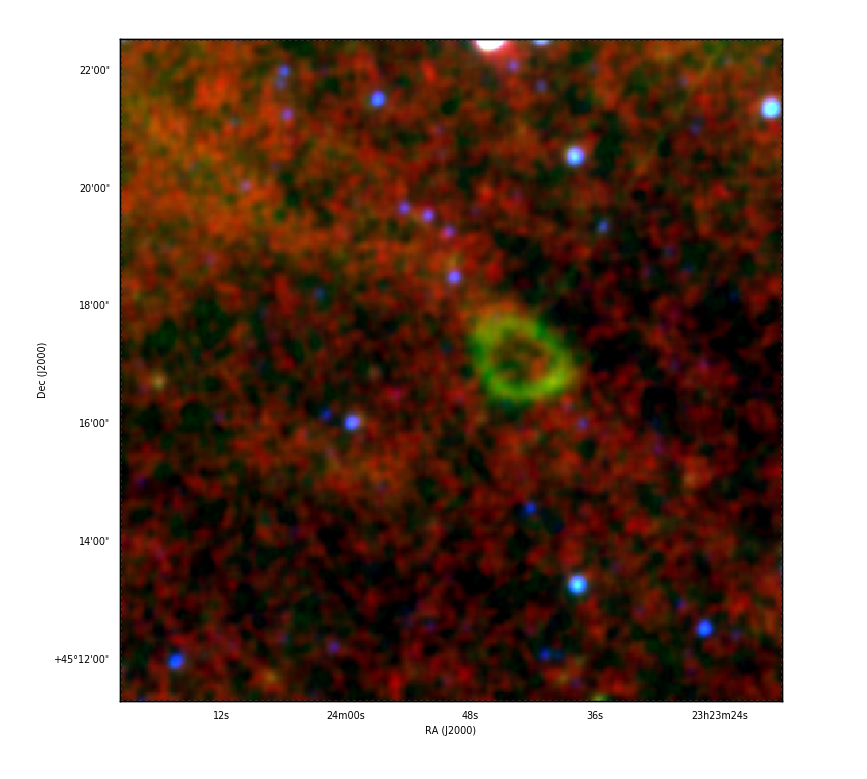
\includegraphics[width=1in]{32280_wise432_rgb.png} & True PN \\ \hline
17907 & NGC 16 & 111.58614 & -34.2072 & 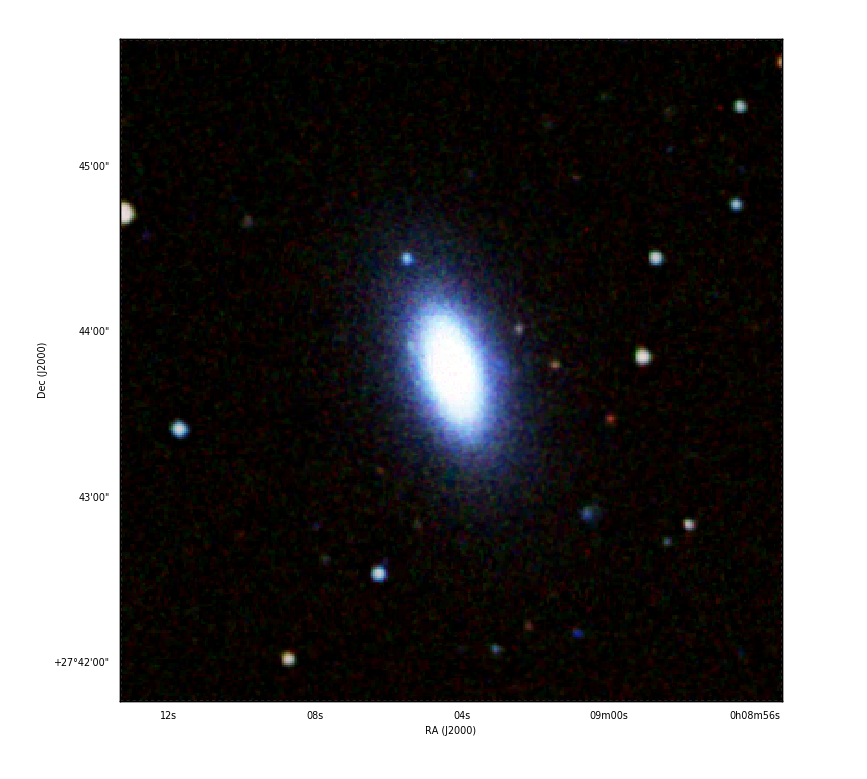
\includegraphics[width=1in]{17907_sss_irb2.png} & Rejected PNe (galaxy) \\ \hline
\end{tabular}
\caption{Subsample of HashDB dataset}

\end{table}


\subsection{Implementation Plan}
% TODO Implementation plan
Our project will be mainly based on using the PyTorch framework. We will take inspiration from our prior work within the course, in addition to writing our own data scraping methods.

In phase one, we will attempt to \textbf{reproduce the baseline model} as described in \citet{awangiskandar2020} by pre-training the InceptionResNetV2 on ImageNet1k, and then performing Linear Probing (LP) using our dataset. As the authors have not publicly published their codebase, we will be heavily adapting and modifying our coursework codebase on LP to create as similar of an implementation as described in the original paper.

We will then further our investigation in phase two, by experimenting with \textbf{Linear Probing then Fine Tuning} (LP-FT) where we will attempt Fine Tuning on our Phase One model. As an initial study, we will attempt to Fine Tune the last three layers of the model, but this may still change depending on the performance yields and resources available to us at the time. This phase is beyond the scope of the original paper; we will be writing most of the code to implement this ourselves, taking inspiration from prior work we have done through this course.

Finally, in phase three, we will experiment with implementing \textbf{Pseudo-labeling} with our best phase two model as a base, in hopes of further increasing the classification accuracy of our model on unseen data. This phase is once again beyond the scope of the original paper and we will be writing our own implementation of Pseudo-labeling for our dataset.
\newpage
\bibliographystyle{iclr2021}
\bibliography{references}

\end{document}

